\subsection*{Functions as Structure-Preserving Objects}
\label{subsec:functions-as-structure-preserving-objects}

\begin{definitionbox}{Definition (Function)}
\begin{definition}[Function]
\label{def:alg-function}
Let $A$ and $B$ be sets.
A \textbf{function} from $A$ to $B$ is a relation $f \subseteq A \times B$
such that:
\begin{enumerate}[label=(\roman*)]
  \item $\forall a \in A,\; \exists b \in B,\; (a,b) \in f$;
  \item if $(a,b_1) \in f$ and $(a,b_2) \in f$, then $b_1=b_2$.
\end{enumerate}
We write $f:A\to B$ and $f(a)=b$ in place of $(a,b)\in f$.
\end{definition}
\end{definitionbox}

\begin{remark*}[Standard quantified statement]
\[
\operatorname{Function}(f,A,B)
\quad\Longleftrightarrow\quad
\forall a \in A,\; \exists!\, b \in B \text{ such that } (a,b)\in f.
\]
\end{remark*}

\begin{remark*}[Definition predicate reading]
$f$ is a function from $A$ to $B$ exactly when every input in $A$ has exactly
one output in $B$.
\end{remark*}

\begin{remark*}[Negated quantified statement]
\[
\neg\operatorname{Function}(f,A,B)
\Longleftrightarrow
\exists a\in A\text{ with no output in }B
\lor
\exists a\in A\text{ with two distinct outputs in }B.
\]
\end{remark*}

\begin{figure}[htbp]
  \centering
  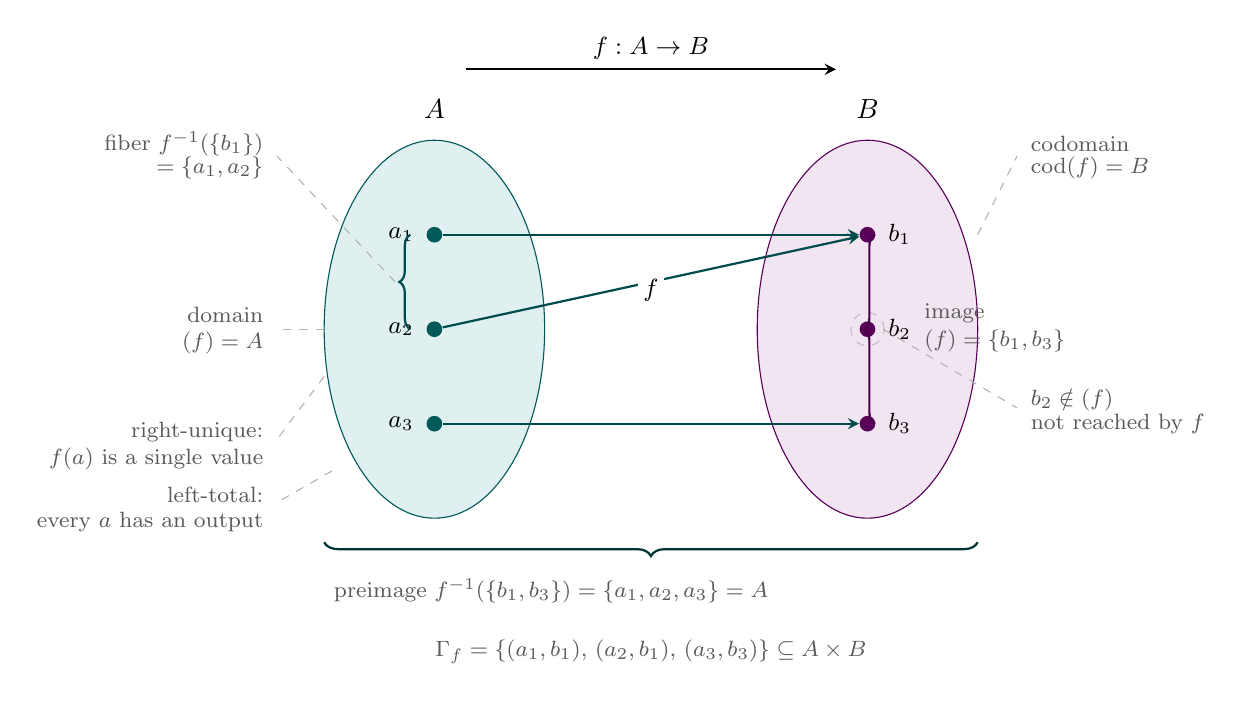
\begin{tikzpicture}[
    >=stealth,
    dot/.style     = {circle, fill, inner sep=2pt},
    teal/.style    = {draw=teal!70!black,  fill=teal!12},
    purple/.style  = {draw=violet!70!black, fill=violet!10},
    lbl/.style     = {font=\small},
    ann/.style     = {font=\footnotesize, text=gray!70!black},
    leader/.style  = {gray!60, dashed, thin},
    arr/.style     = {->, thick, teal!60!black},
    brace/.style   = {decorate,
                      decoration={brace, amplitude=4pt, raise=3pt},
                      thick, violet!60!black}
  ]
  \draw[teal]   (0,0)   ellipse (1.4cm and 2.4cm);
  \draw[purple] (5.5,0) ellipse (1.4cm and 2.4cm);

  \node[font=\normalsize\bfseries] at (0,    2.8) {$A$};
  \node[font=\normalsize\bfseries] at (5.5,  2.8) {$B$};

  \node[dot, teal!70!black] (a1) at (0,  1.2) {};
  \node[dot, teal!70!black] (a2) at (0,  0)   {};
  \node[dot, teal!70!black] (a3) at (0, -1.2) {};
  \node[lbl, left=4pt] at (a1) {$a_1$};
  \node[lbl, left=4pt] at (a2) {$a_2$};
  \node[lbl, left=4pt] at (a3) {$a_3$};

  \node[dot, violet!70!black] (b1) at (5.5,  1.2) {};
  \node[dot, violet!70!black] (b2) at (5.5,  0)   {};
  \node[dot, violet!70!black] (b3) at (5.5, -1.2) {};
  \node[lbl, right=4pt] at (b1) {$b_1$};
  \node[lbl, right=4pt] at (b2) {$b_2$};
  \node[lbl, right=4pt] at (b3) {$b_3$};

  \draw[gray!50, dashed, thin] (b2) circle (6pt);
  \draw[arr] (a1) -- (b1);
  \draw[arr] (a2) -- (b1);
  \draw[arr] (a3) -- (b3);
  \node[fill=white, inner sep=2pt, font=\small\bfseries] at (2.75, 0.5) {$f$};
  \draw[->, thick] (0.4, 3.3) -- node[above, font=\small\bfseries] {$f : A \to B$} (5.1, 3.3);

  \draw[leader] (-1.4, 0) -- (-2.0, 0);
  \node[ann, anchor=east] at (-2.05, 0.18) {domain};
  \node[ann, anchor=east] at (-2.05,-0.18) {$\dom(f) = A$};
  \draw[leader] (-1.3,-1.8) -- (-2.0,-2.2);
  \node[ann, anchor=east] at (-2.05,-2.1) {left-total:};
  \node[ann, anchor=east] at (-2.05,-2.45) {every $a$ has an output};
  \draw[leader] (-1.4, -0.6) -- (-2.0, -1.4);
  \node[ann, anchor=east] at (-2.05,-1.3)  {right-unique:};
  \node[ann, anchor=east] at (-2.05,-1.65) {$f(a)$ is a single value};

  \draw[leader] (6.9,  1.2) -- (7.4,  2.2);
  \node[ann, anchor=west] at (7.45, 2.35) {codomain};
  \node[ann, anchor=west] at (7.45, 2.05) {$\mathrm{cod}(f) = B$};
  \draw[brace] (5.7, -1.2) -- (5.7,  1.2);
  \node[ann, anchor=west] at (6.1,  0.2) {image};
  \node[ann, anchor=west] at (6.1, -0.15) {$\im(f) = \{b_1, b_3\}$};
  \draw[leader] (5.7, 0) -- (7.4, -1.0);
  \node[ann, anchor=west] at (7.45,-0.9)  {$b_2 \notin \im(f)$};
  \node[ann, anchor=west] at (7.45,-1.2)  {not reached by $f$};

  \draw[decorate,
        decoration={brace, amplitude=4pt, raise=3pt},
        thick, teal!60!black]
    (-0.2, 0) -- (-0.2, 1.2);
  \draw[leader] (-0.5, 0.6) -- (-2.0, 2.2);
  \node[ann, anchor=east] at (-2.05, 2.35) {fiber $f^{-1}(\{b_1\})$};
  \node[ann, anchor=east] at (-2.05, 2.05) {$= \{a_1, a_2\}$};

  \draw[decorate,
        decoration={brace, amplitude=5pt, raise=3pt, mirror},
        thick, teal!40!black]
    (-1.4,-2.6) -- (6.9,-2.6);
  \node[ann, anchor=north west] at (-1.4,-3.05)
    {preimage $f^{-1}(\{b_1,b_3\}) = \{a_1,a_2,a_3\} = A$};
  \node[ann] at (2.75,-4.1)
    {$\Gamma_f = \{(a_1,b_1),\,(a_2,b_1),\,(a_3,b_3)\} \subseteq A \times B$};
\end{tikzpicture}

  \caption{Vocabulary of a function $f:A\to B$.}
  \label{fig:function-vocabulary}
\end{figure}

\begin{remark*}[Interpretation]
A function assigns exactly one output in $B$ to every input in $A$.
In algebra, functions become structure-preserving objects when they are
required to respect specified operations, relations, or constants.
\end{remark*}

\begin{dependencies}
\begin{itemize}
  \item \hyperref[def:binary-relation]{Binary Relation}
  \item \hyperref[def:domain-codomain]{Domain and Codomain}
\end{itemize}
\end{dependencies}
